\documentclass{article}
\usepackage{amsmath}
\usepackage{amssymb}
\usepackage{graphicx}
\usepackage{hyperref}
\usepackage[version=4]{mhchem}

\title{Example 6}
\date{}

\begin{document}
\maketitle

(IMO) A circle has center on the side \(A B\) of the cyclic quadrilateral \(A B C D\). The other three sides are tangent to the circle. Prove that \(A D+B C=A B\).

Solution:
Connect \(O E, O G, O F\). Extend \(O F\) to meet the extension of \(G C\) to \(N\).\\
Let the radius of the circle be \(r\). Let \(\angle N C F=\alpha\).\\
\centering
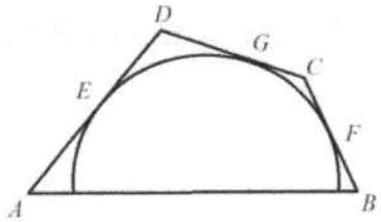
\includegraphics[width=\textwidth]{images/149.jpg}\\
\(\angle C N F=\beta . \alpha+\beta=90^{\circ}\).\\
Since quadrilateral \(A B C D\) is cyclic, \(\angle N C F=\angle A\)\\
\(=\alpha\).\\
Thus Rt \(\triangle A E O \sim\) Rt \(\triangle C F N\).\\
So \(C F=\frac{A E \times F N}{r}\).\\
We know that \(\angle O G N=90^{\circ}\). So \(\angle G O N=\alpha\).\\
\centering
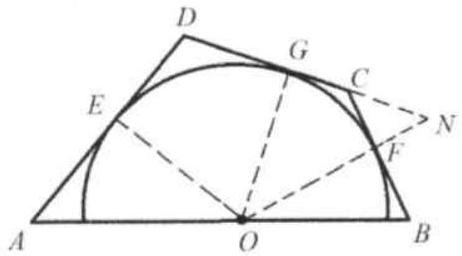
\includegraphics[width=\textwidth]{images/149(2).jpg}

We know that \(\angle O E A=90^{\circ}\). So \(\angle E O A=\beta\).\\
Thus Rt \(\triangle O G N \sim\) Rt \(\triangle A E O\).\\
So \(O A=\frac{A E \times O N}{O G}=\frac{A E(r+F N)}{r}\)\\
\(=A E+\frac{A E(F N)=A E+C F}{r}\).\\
\centering
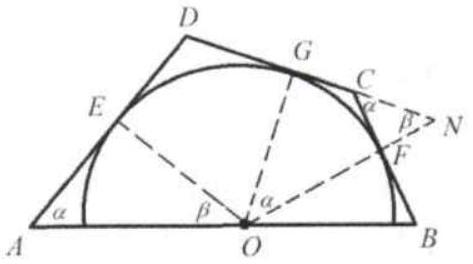
\includegraphics[width=\textwidth]{images/149(1).jpg}

Similarly, \(O B=B F+D E\).\\
Thus \(A B=O A+O B=A E+C F+B F+D E=A D+B C\).



\end{document}
